%!TEX root = ../../report.tex
\chapter{Implementation} % (fold)
\label{cha:implementation}
The chapter \ref{cha:analysis} is meant for studying conceptual designs of the platform, and from the chapter \ref{cha:mathematical_model} some mathematical constraints are obtained, whilst the chapter \ref{cha:design} is where the robot is designed in its electronic, mechanical and control facets.
This chapter is dedicated to explain the process of creating those designs and create real working components.
From the important role of emerging low-cost technologies like FFF 3D printing up to the creation of custom PCBs for reducing the weight of the robot, the following sections are meant to explain the process of creation and acquisition (from the several providers) but following always a criteria of security, constrained budget and feasibility for maintenance and futures improvements.

%!TEX root = ../../../report.tex
\section{3D printing} % (fold)
\label{sec:3d_printing}
The parts modeled for the project and shown in section \ref{sub:computer_aided_design}, have been printed using Fused Filament Fabrication (FFF).
The 3D printer used is a M Prime One \footnote{https://github.com/M-Prime/M\_Prime\_One} with a 0.4 mm noozle.
All the parts have been printed at 0.2 mm layer height.

The use of this technology is justify by the fact that makes the iterative process between design and manufacturing both fast and cheap. \todo{Fast and low-cost prototyping}
All the parts have been individually adjusted until the clearances have been as expected.
Furthermore, this enable the user not only to replicate the parts with out any considered extra cost, but allows the robot to be easily replicated in other places.

When manufacturing, some of the parts have needed material support.
\todo{Why the material support? Tell how you've managed to print the most complex stuff}
The figure \ref{fig:photo_material_support} depicts two feet, one with material support and the other with it removed.
In the figure \ref{fig:photo_3d_printed} a detail of actual parts 3D printed and assembled in the robot are shown.

\begin{figure}[ht]
    \centering
    \begin{subfigure}[b]{0.49\textwidth}
        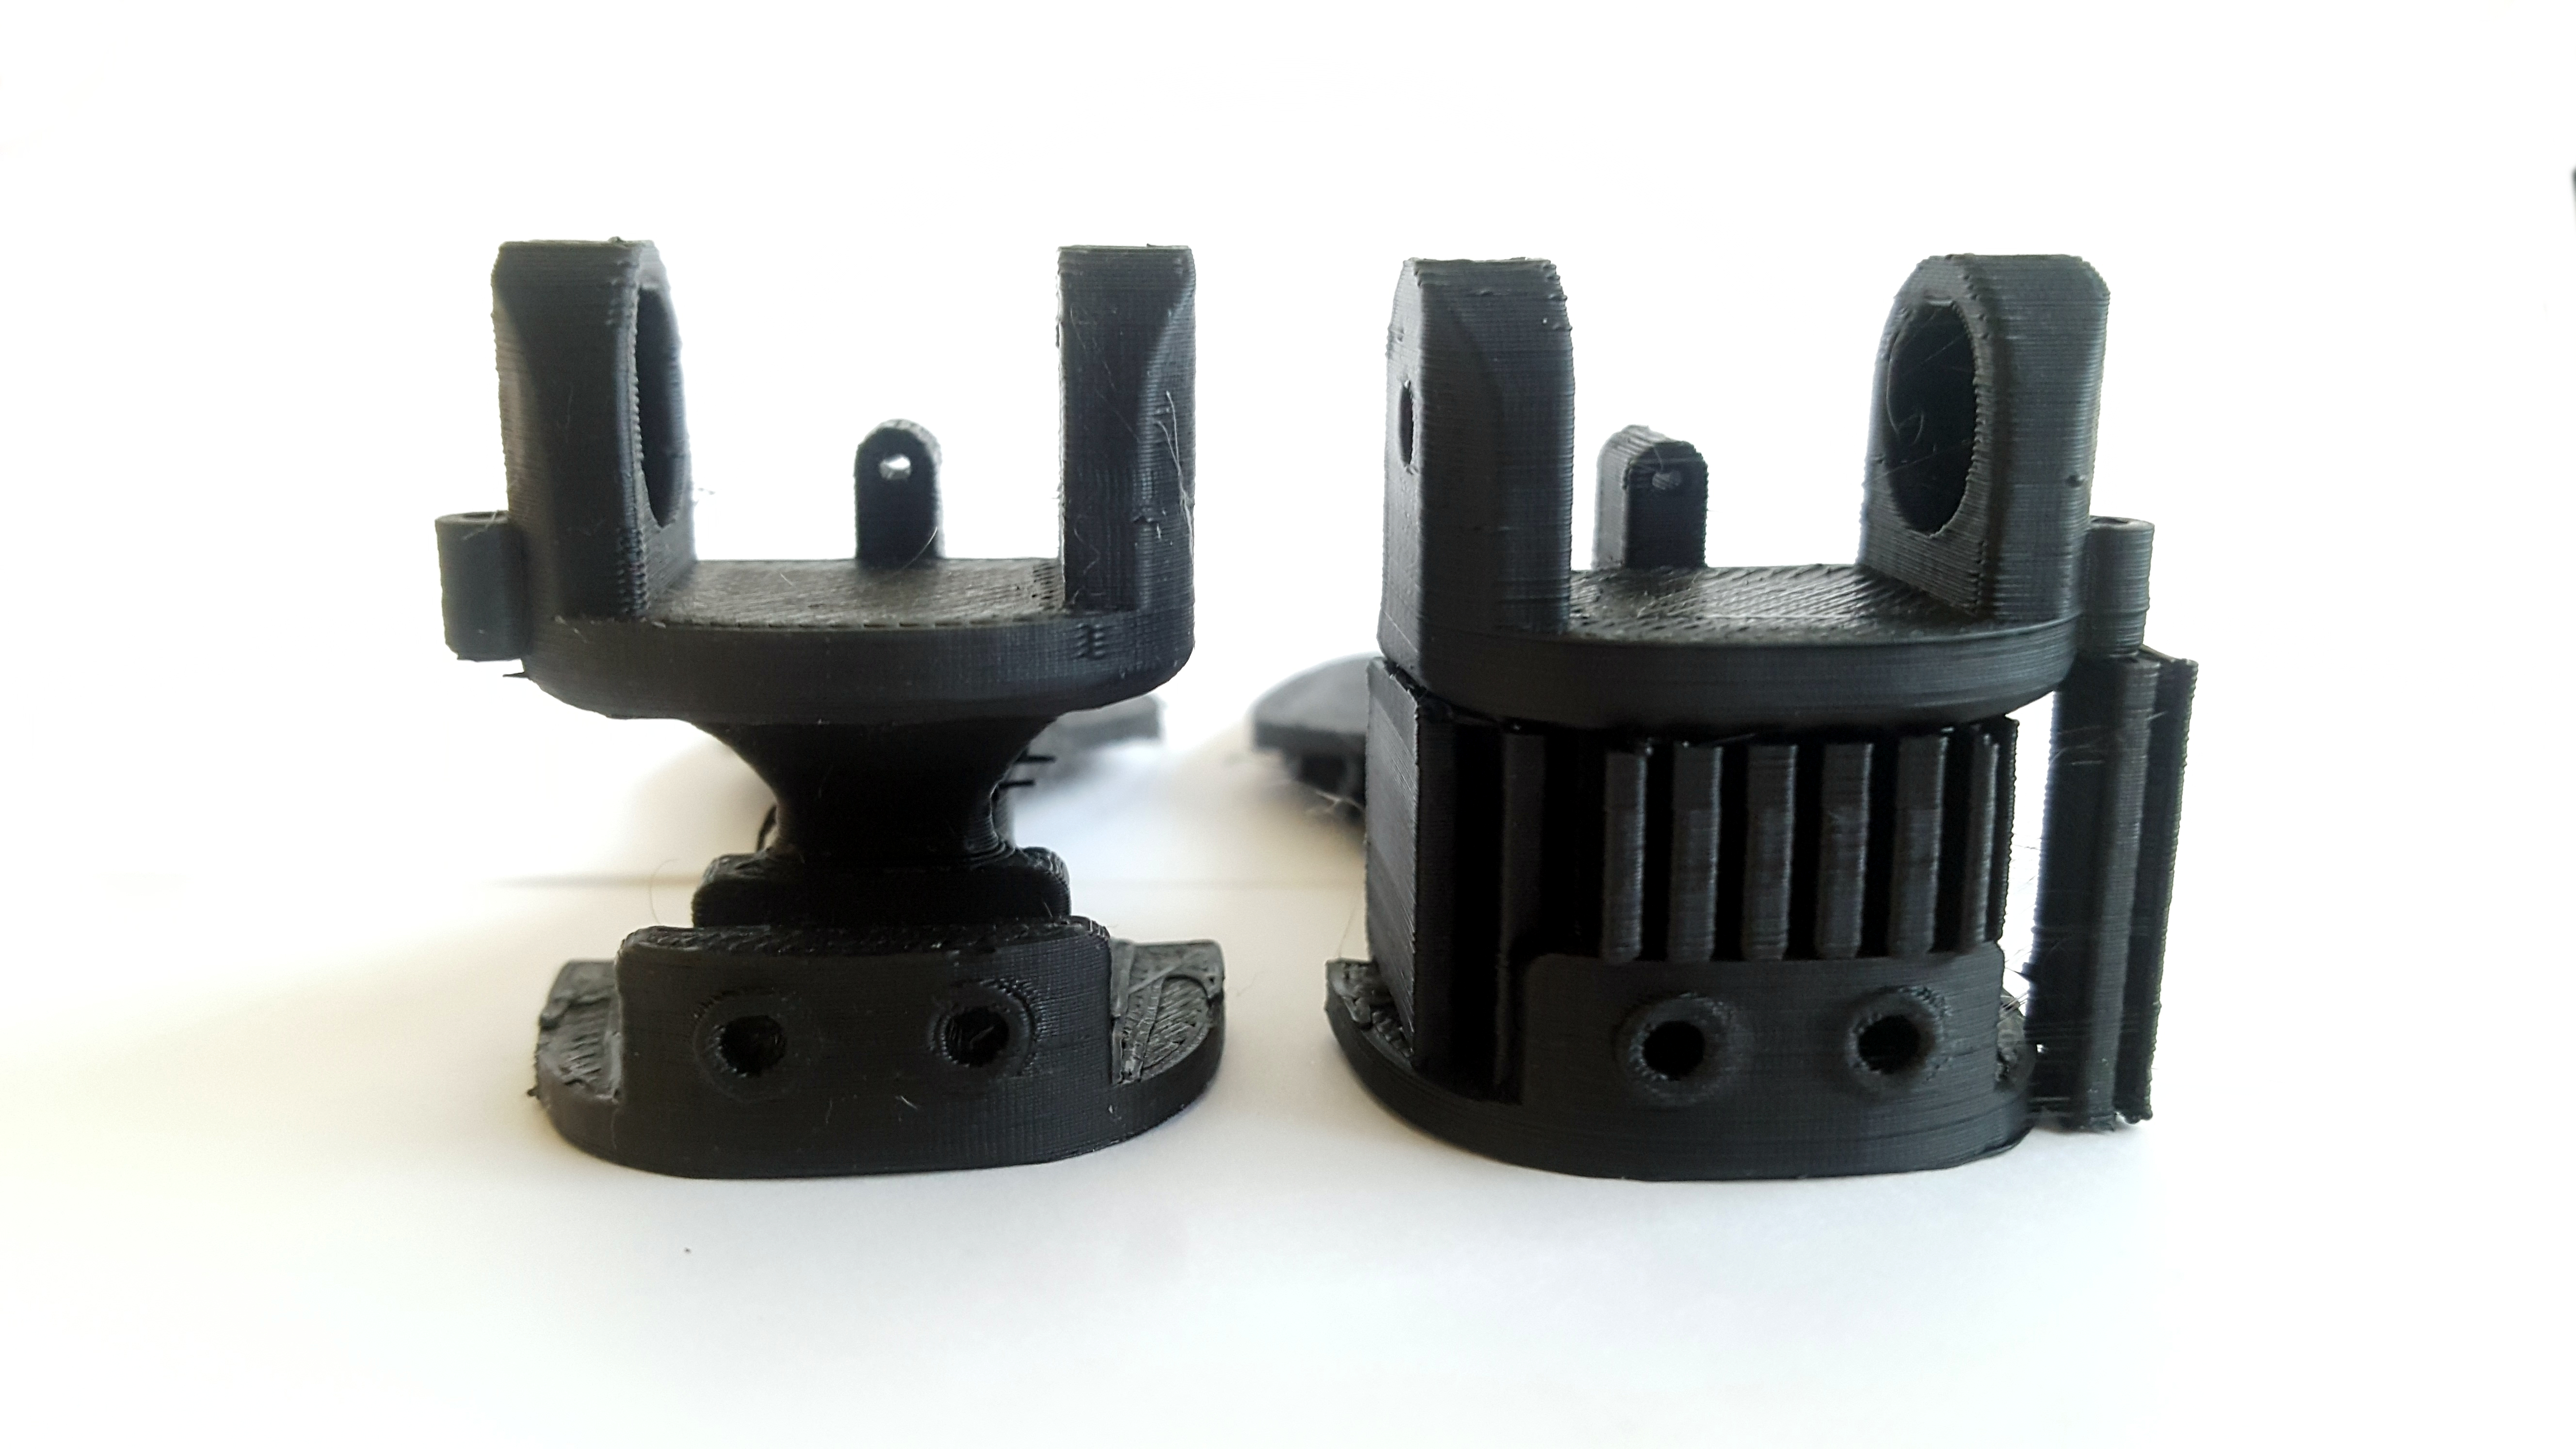
\includegraphics[width=\textwidth]{figures/photo_material_support.jpg}
        \caption{Feet with and without material support}
        \label{fig:photo_material_support}
    \end{subfigure}
    \begin{subfigure}[b]{0.49\textwidth}
        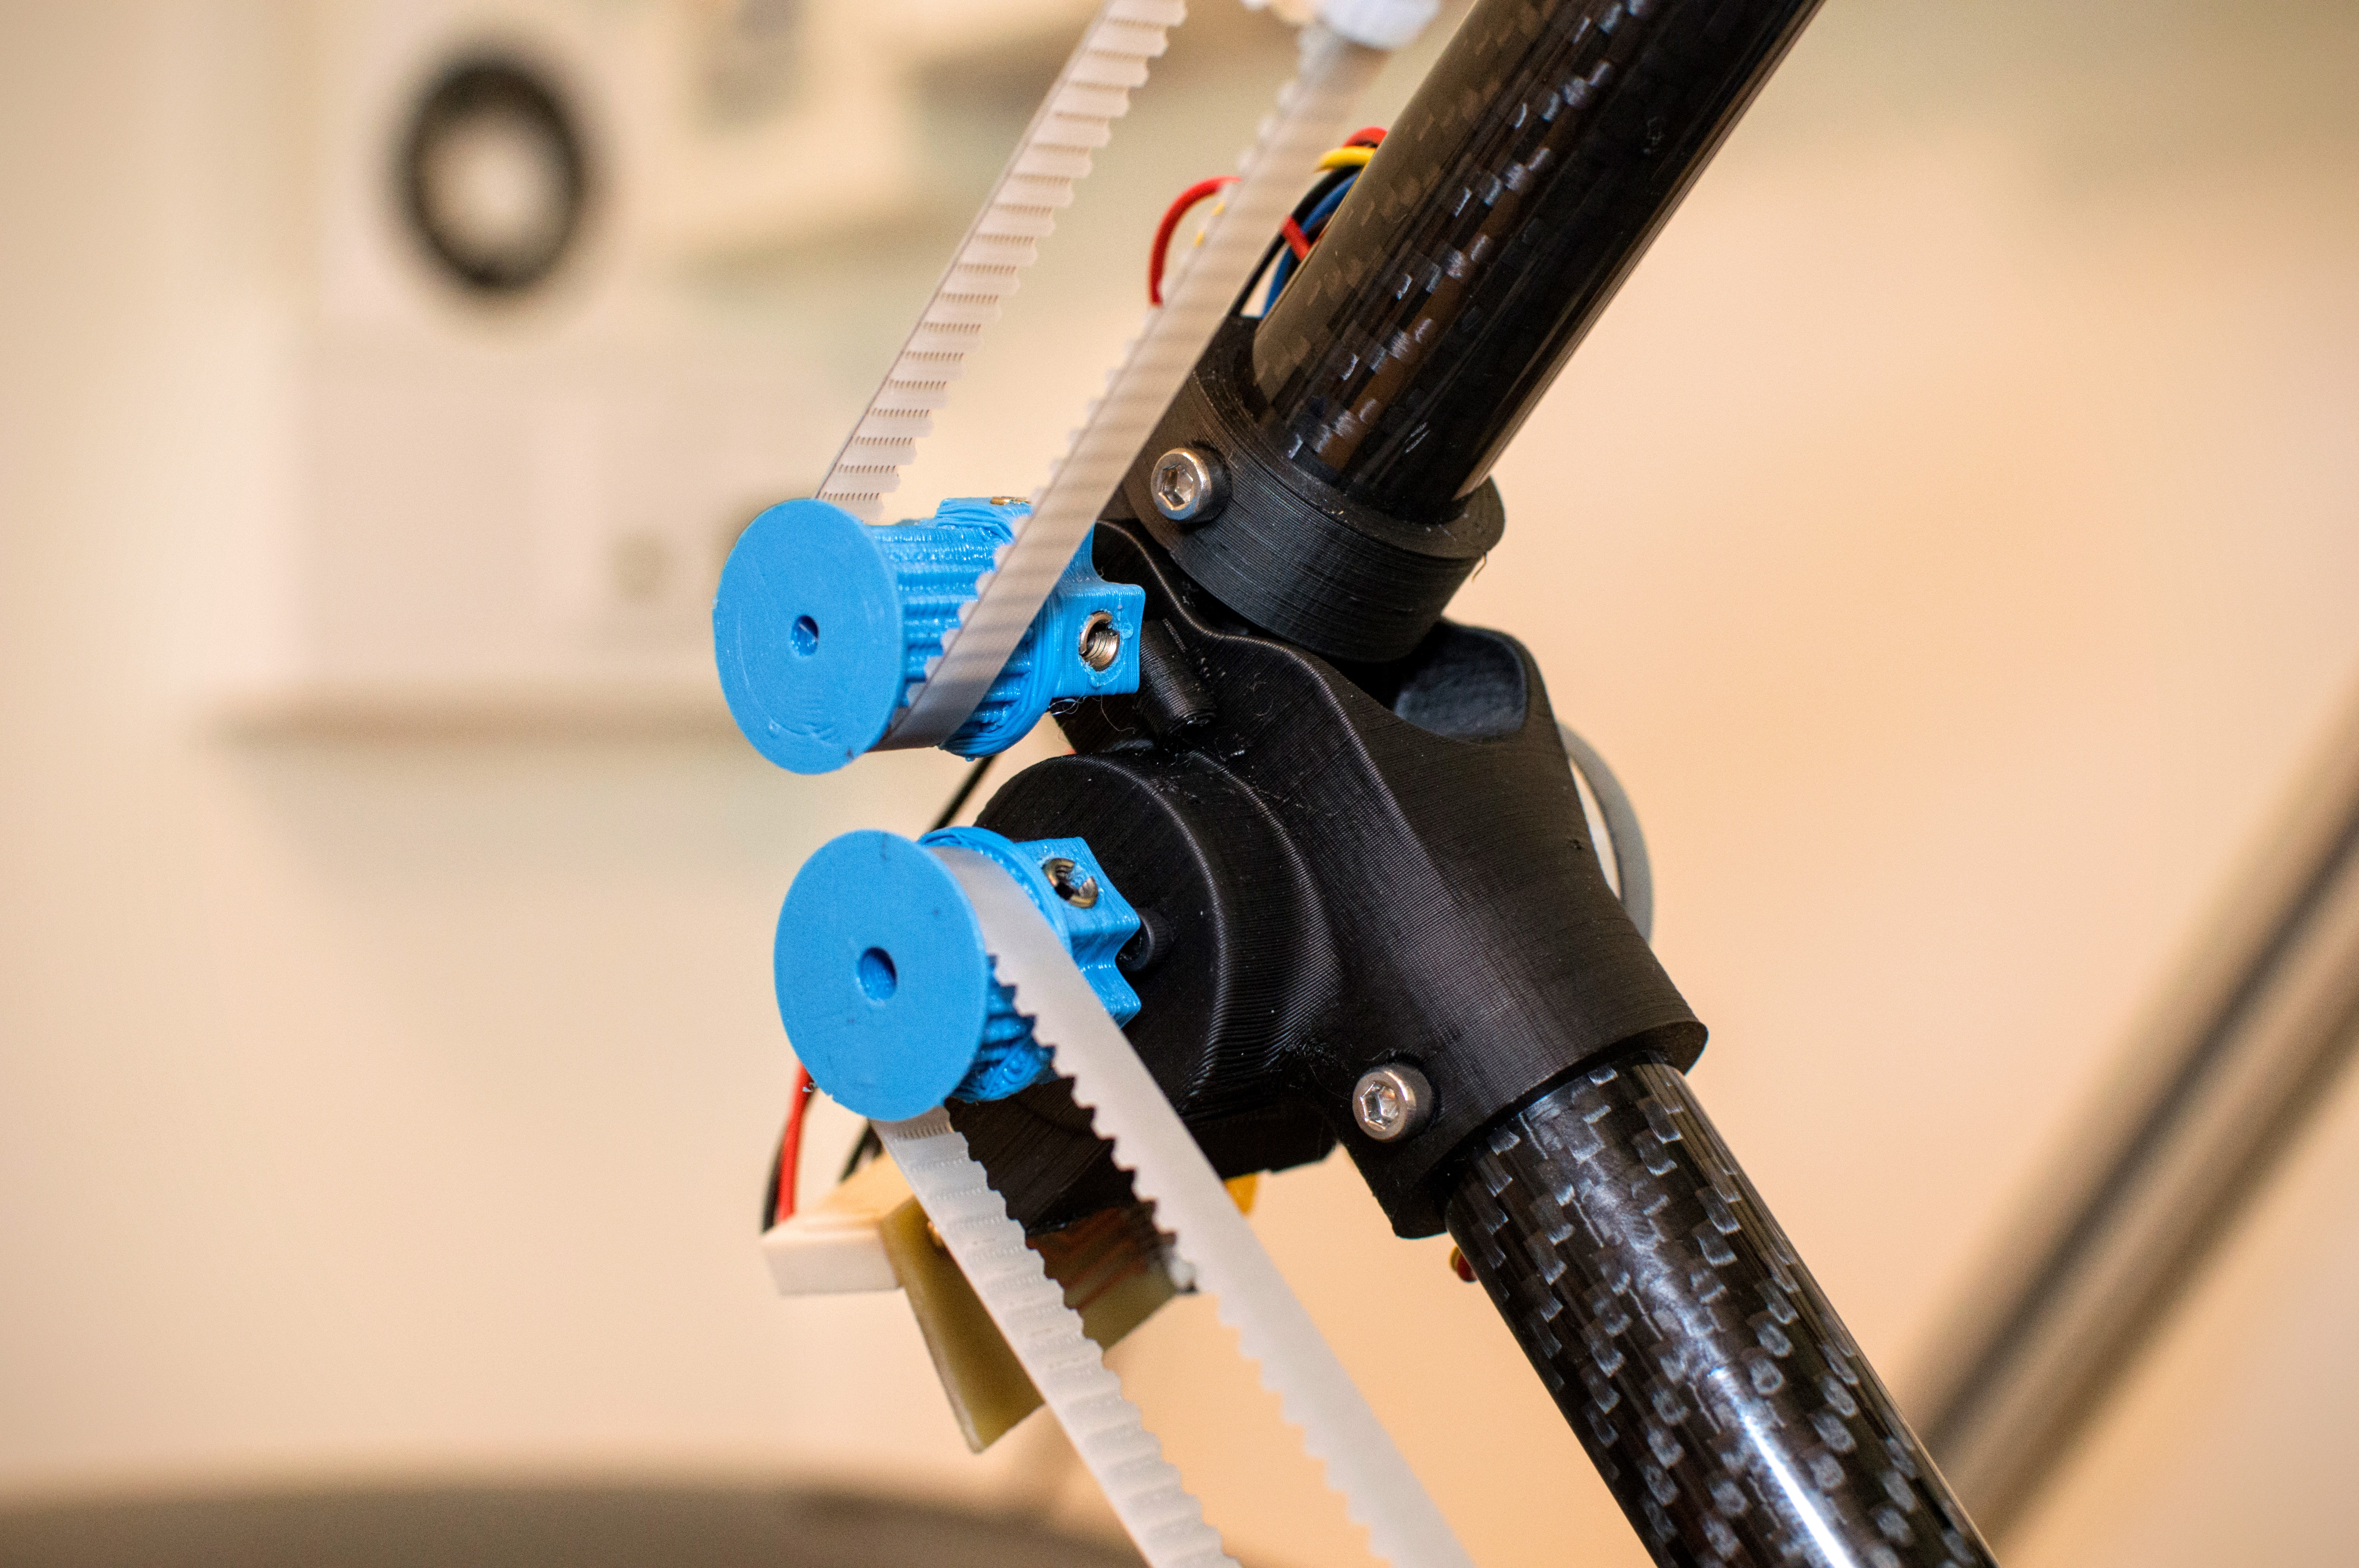
\includegraphics[width=\textwidth]{figures/photo_3d_printed.jpg}
        \caption{Detail of 3D printed parts assembled}
        \label{fig:photo_3d_printed}
    \end{subfigure}
\end{figure}

  \subsection{Arc compensation} % (fold)
  \label{sub:arc_compensation}
  For the CAD models of the 3D printed parts, the clearances of the internal holes have been adjusted following \cite{arc_compensation}.
  The undersizing of internal holes is a common problem in this sort of technology due to the lack of information of the common-used exporting format: the STL.
  This only contains the 3D model expressed as a set of external triangles, which difficult the correction of malformations inherent to the technology.

  In the case of the Fused Filament Fabrication (FFF), the material is extruded equally in both sides of the arc, as shown in \ref{fig:arc_compensation}. 
  However, in the side of the smaller curve, less material is needed.
  This correction can be calculated with:

  \todo{Label and reference the equations}
  $$ r=\frac{t+\sqrt{t^2+4R^2}}{2}$$

  being:
  \begin{enumerate}
    \item t: noozle diameter
    \item R: desired internal hole radius
    \item r: corrected radius
  \end{enumerate}
  As an example, Klee suggests an internal hole of 4.4 mm in the case of the selected nuts \cite{klee}. Thus, the diameter in the CAD model has been adjusted for this data and a noozle of 0.4 mm. The result is then:
  $$ d=2r=\frac{t+\sqrt{t^2+4R^2}}{2}=0.4+\sqrt{0.4^2+4*2.2^2}=4.81$$

  \begin{figure}[tb]
    \centering
    \includegraphics[width=0.5\textwidth]{figures/Arc-compensation}
    \caption{Technical representation of the generated arc when using FFF technology}
    \label{fig:arc_compensation}
  \end{figure}
  % subsection arc_compensation (end)

% section 3d_printing (end)
%!TEX root = ../../../report.tex
\section{Machining} % (fold)
\label{sec:machining}
Along with 3D printing, other parts have needed to be machined.
Though its allows the creating of complex geometries, the 3D printers used have a limited printing volume.
Additionally, the mechanical properties given by the PLA do not satisfy all the needs of the used parts.
The rods of the axis, the beams used to create the structure, the carbon fiber tubes are some examples of this requirements of size and mechanical stress.
Special attention has been paid to the symmetry during the construction following the design criteria established in \ref{sec:physical_properties}.

This materials usually come in a raw format that must be then modified in order to get the desired component.
As an example, the rods came in bars of one meter that have been cut and filed according the design.
Other example are the carbon fiber tubes.
These have been designed to carry the wiring inside them.
Thus some holes have been performed in the bottom and top part of the tube in order to insert them.
Knowing that this kind of operations is human error prone, non-critical parts have been machined or no such it can affect to the correct behavior of the device.
Furthermore, the actuation has always tried to be as much correct as possible and always following the appropriate security rules.
The drawings for such parts are included as appendices in \ref{app:mechanical_drawings}.

% section machining (end)
%!TEX root = ../../../report.tex
\section{PCBs and wiring} % (fold)
\label{sec:pcbs_and_wiring}

% section pcbs_and_wiring (end)
%!TEX root = ../../../report.tex
\section{Providers} % (fold)
\label{sec:providers}
In addition to the 3D printed and machined parts, other items have been bought from providers.
The providers have been selected based on previous shoppings made by the Mærsk Mc-Kinney Møller Institute.
All the needed items that could have followed an standard have been chosen. 
As an example, the robot only needs three types of screws and one kind of bearings.
The components are easily found and are not rare items that increase the price of the robot.
A list with all the components bought and its providers is attached as an appendix in \ref{app:order_list}.
% section providers (end)
%!TEX root = ../../../report.tex
\section{Assembly} % (fold)
\label{sec:assembly}
Due to basically all the parts have been somehow connected with a 3D printed parts, and all the tolerances of these have been adjusted individually, the assemble process has been found easy and fast.
The mounting processes has shown to be rapid enough to change some of the parts, as the springs, within minutes.
Furthermore, if any part breaks its creation and replacement is easy enough to reduce the maintenance time and be considered it as one of the main points of the whole platform.
The tension of the belts have been adjusted experimentally as explained in the section \ref{sub:pulleys_and_belts} using the zip ties installed.
In the figure \ref{fig:photo_robot_walking}, the complete robot assembled is shown while in the figure \ref{fig:photo_dacbot}, a size comparison between the Dacbot \cite{dacbot1} and RuBi can be done.

\begin{figure}[ht!]
    \centering
    \begin{subfigure}[b]{0.49\textwidth}
        \includegraphics[width=\textwidth]{figures/photo_robot_walking.jpg}
        \caption{RuBi assembled}
        \label{fig:photo_robot_walking}
    \end{subfigure}
    \begin{subfigure}[b]{0.49\textwidth}
        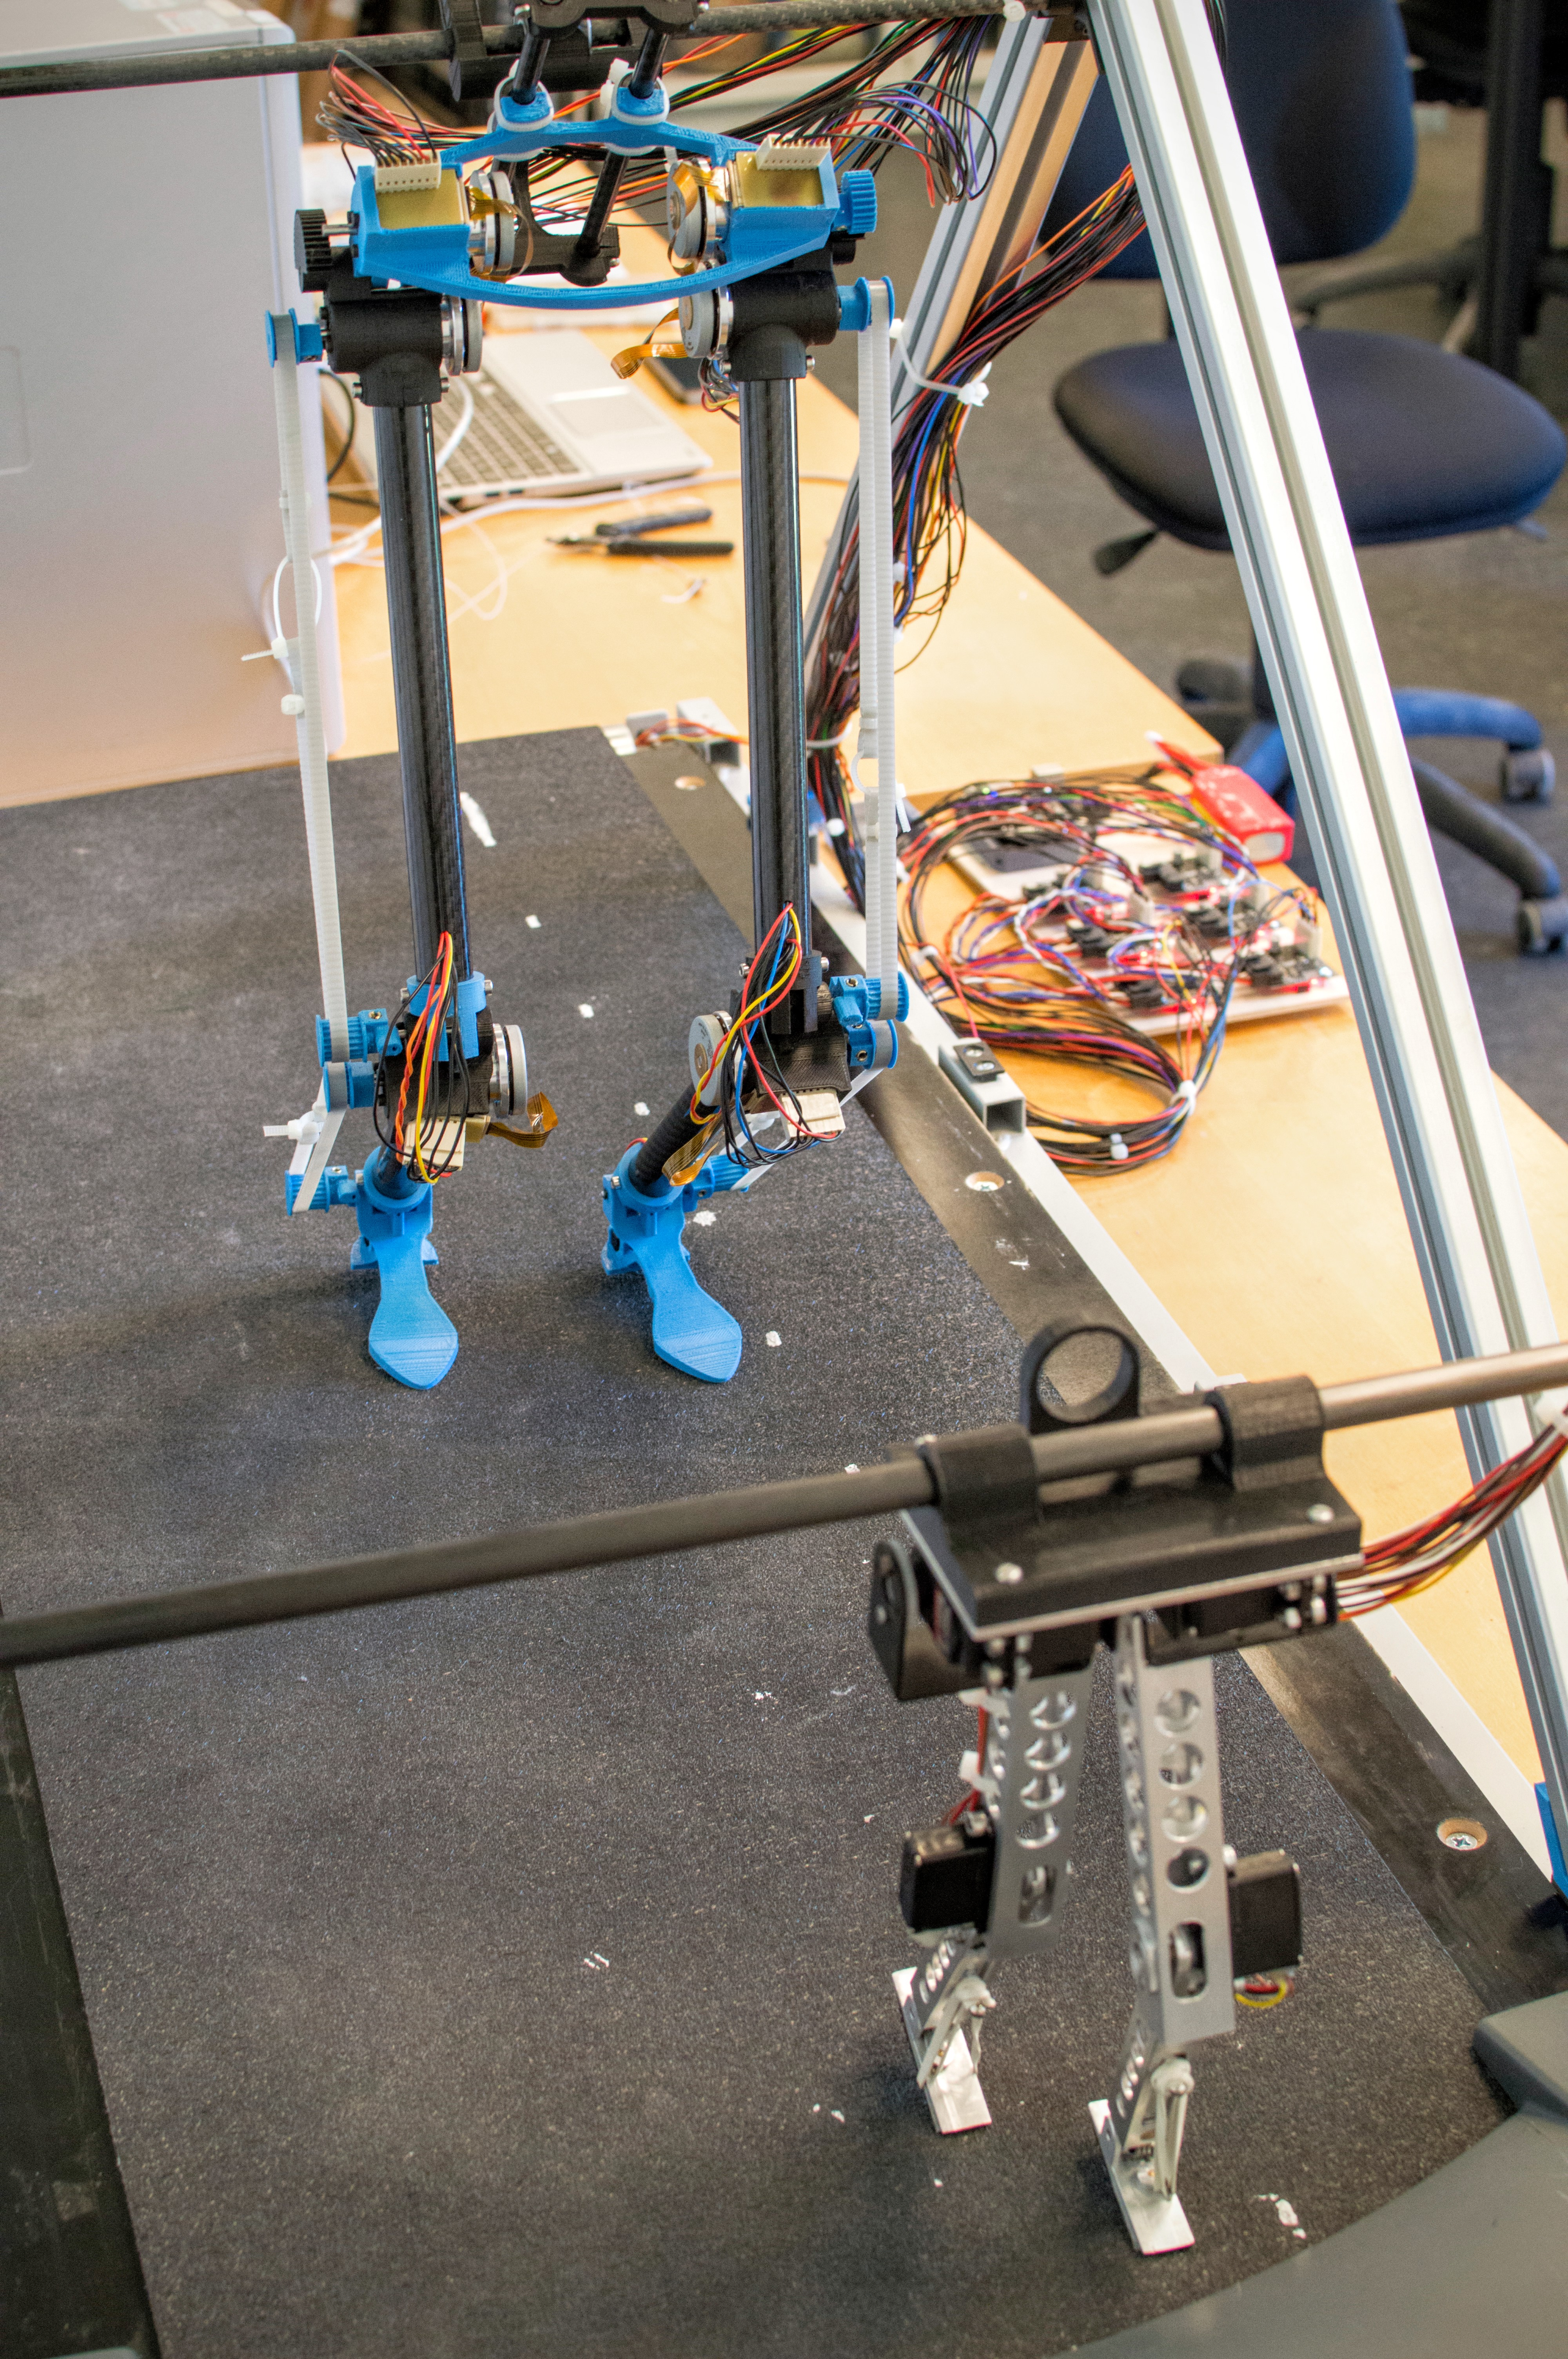
\includegraphics[width=\textwidth]{figures/photo_dacbot.jpg}
        \caption{RuBi and Dacbot over the same treadmill}
        \label{fig:photo_dacbot}
    \end{subfigure}
\end{figure}    
% section assembly (end)
%!TEX root = ../../../report.tex
\section{How to bring up the robot} % (fold)
\label{sec:how_to_bring_up_the_robot}
In order to bring up the robot, a battery has to power it and the computer must be started.
It will automatically create a Wi-Fi hotspot called \textit{RuBi} where the user can connect to.
From this moment, the robot should be able to receive motor commands.
If not, the IP in the \textit{locokit\_hw} has to be changed according to the stablished in the host.
In the guest, open a new terminal and run:

\begin{lstlisting}
roslaunch rubi_bringup rubi_bringup.launch
\end{lstlisting}

ROS Control will be loaded along with the locokit hardware interface and the controllers can move the real robot.
% section how_to_bring_up_the_robot (end)

% chapter implementation (end)